\begin{figure}[t]
 	\centering
	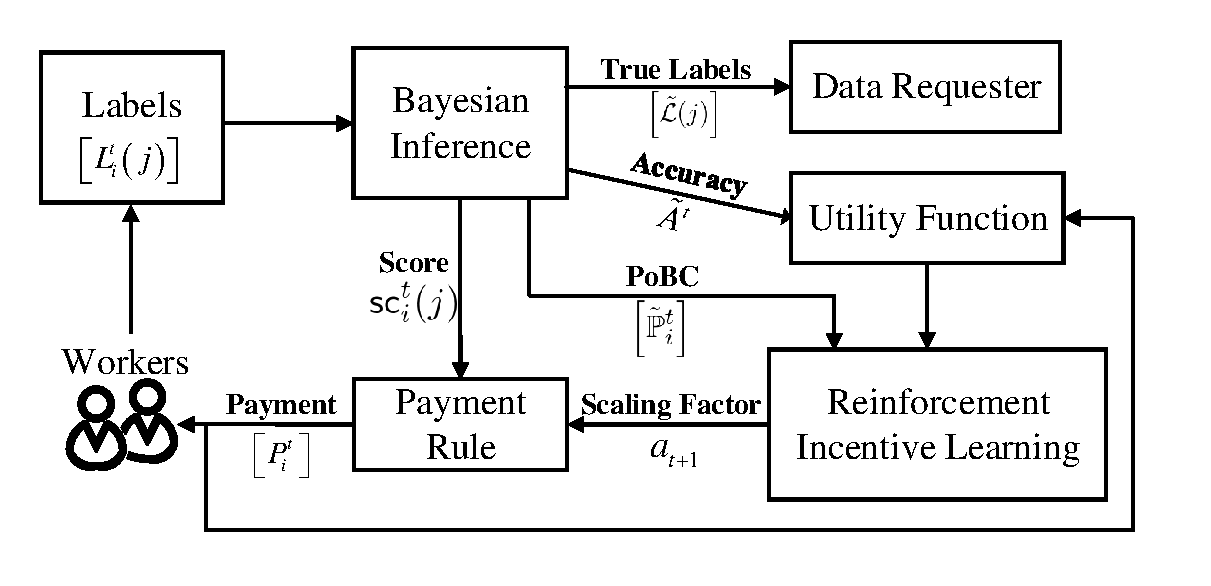
\includegraphics[width=0.48\textwidth]{image/Architecture}
	\vspace*{-8mm}
    \caption{\label{figure:layout} Layout of our incentive mechanism.}
\end{figure}
\section{Incentive Mechanism for Crowdsourcing}
We present the overall layout of our mechanism in Figure~\ref{figure:layout}, where estimated values are denoted with over-the-head tildes. In this section, we formally introduce the three main components of our design: payment rule, bayesian inference and reinforcement learning.

The payment rule is designed to ensure that reporting truthfully and exerting high efforts  is the payment-maximizing strategy for all workers at any given time. Besides, our incentive mechanism as a whole guarantees that this is also the payment-maximizing strategy for all workers in the long run. We kindly refer readers to Section~\ref{analysis} for the theoretical proof. This property prevents clever manipulations from workers, which bring more long-term benefits to them by sacrificing short-term ones, or the other way around. 
By doing so, we wish to induce workers to generate high-quality labels. %and thus improve the label accuracy. 
The Bayesian inference algorithm is responsible for estimating the true labels, workers' PoBCs and the aggregate label accuracy from the collected labels at each time step. It utilizes soft Dirichlet priors and Gibbs sampling to prevent overestimation of accuracy when workers generate poor-quality labels. The reinforcement learning algorithm adjusts the payment rule based on the historical data of payments, workers' PoBCs and aggregate labels' accuracy, aiming to optimally balance the utility gain from high accuracy and loss from large payments, which corresponds to $F(A^t)$ and $\sum_{i}P_i^t$ in Equation~\ref{equation:utility} respectively.


%Nevertheless, there are three challenges to achieve our design. Firstly, our empirical studies reveal that popular inference algorithms may be heavily biased towards overestimating the accuracy when the quality of labels is very low. For example, when there are $10$ workers and $q_i^t=0.55$, the estimated label accuracy of the EM estimator~\cite{dawid1979maximum,raykar2010learning} stays at around $0.9$ while the real accuracy is only around $0.5$.
%This heavy bias will cause the utility to be miscalculated and thus mislead our reinforcement adjustment.
%To reduce the inference bias, we develop our Bayesian inference algorithm by introducing the soft Dirichlet priors to both the true labels and workers' PoBCs.
%In this case, the posterior distribution cannot be expressed as any known distributions, which motivates us to derive the explicit posterior distribution at first and then employ Gibbs sampling to conduct inference.
%{\color{red}Secondly, the reinforcement adjustment expects the utility to be accurately calculated so that the direction of adjustment is clear.
%However, both the label accuracy and workers' PoBCs in our incentive mechanism are corrupted by noise.
%Considering that these estimates are calculated as an average over $M$ tasks, the central limit theorem ensures that the inference noise approaches the Gaussian distribution.
%Therefore, to overcome the inference noise, we develop our reinforcement adjustment algorithm based on the Gaussian process.}
%Lastly, the biggest challenge of our study is to prove that our incentive mechanism can ensure that reporting truthfully and exerting high efforts is the payment-maximizing strategy for workers in not only each time step and but also the long term.
%For clarity, we put the theoretical analysis in the next section.
%In this section, we focus on the first two challenges.


%Figure~\ref{Archi} shows the architecture of our incentive framework.
%Different from industrial feedback control systems, crowdsourcing markets require the data requester to announce the incentive mechanism to workers before allocating tasks to workers, which is actually a contract between two sides.
%So, we design our framework as two levels.
%The inner level is the Bayesian incentive mechanism which is always open to workers.
%Its objective is to ensure that reporting truthfully and exerting high efforts are the optimal strategy for all workers at any time step $t$.
%By doing so, we expect that all workers are fully rational and can follow this optimal strategy.
%However, in practice, human workers may not always fully rational and can even learn from the interactions with our mechanism.
%Thus, we develop the outer level, the reinforcement incentive mechanism, which adjusts the scaling level $a^t$ of our Bayesian mechanism to maximize the long-term utility of the data requester.
%Meanwhile, our reinforcement incentive mechanism must also ensure that reporting truthfully and exerting high efforts are the optimal strategy for workers in the long term.
%In this way, we can prevent the manipulation of any single worker.




\subsection{Payment Rule}
Suppose, at time step $t$, worker $i$ finishes $m^{t}_i$ tasks. For any given time $t$, all $m^{t}_i$s as a whole must satisfy $\sum_i m^t_i= M$. Then the payment for worker $i$ at time $t$ is
\begin{equation}
P^t_i=m^t_i\cdot (a^t \textsf{sc}^{t}_i+b)\;\; , \;\; \textsf{sc}^{t}_i = \tilde{\mathbb{P}}^{t}_i - 0.5
\label{equation:payment}
\end{equation}
where $\textsf{sc}$ denotes worker $i$'s score, which is proportional to his or her PoBC $\tilde{\mathbb{P}}^{t}_i$ calculated by the Bayesian inference algorithm. $b\geq 0$ is a constant representing the fixed base payment even if the worker purely returns random labels. We use $a^t \in \mathcal{A}$ to denote the scaling factor, determined by our reinforcement adjustment algorithm at the beginning of every time step $t$. We further assume $\mathcal{A}$ is a finite set.


\subsection{Bayesian Inference}
%An accurate inference algorithm, which is responsible for estimating $L^{t}(j)$, $p^t_i$ and $A^t$, is the foundation of our framework. There have been many inference algorithms developed in the literature~\cite{zheng2017truth}. Among them, two popular ones are the EM estimator~\cite{dawid1979maximum} and the variational inference estimator~\cite{liu2012variational}.
%However, our empirical studies in Figure~\ref{BIM1} reveal that these iterative estimators, which may converge to the local optimum, will be heavily biased when the quality of labels is very low.
%Thus, we employ the similar Dirichlet priors as the variation inference estimator but explicitly derive the posterior distribution of true labels rather than relying on the evidence lower bound~\cite{blei2017variational}.
%Then, we use Gibbs sampling to efficiently sample the posterior distribution to calculate the estimates of $L^{t}(j)$, $p^t_i$ and $A^t$.

%since the EM estimator may converge to the local optimum.
%On the other hand, sampling-based Bayesian inference algorithms, for example Gibbs sampling, are computationally very expensive, even though they use the explicit posterior distribution and can avoid the inference bias.
%Especially, workers' scores are continuous variables, which will significantly slow down the convergence speed.
%Therefore, to the best of my knowledge, sampling-based Bayesian inference is never used for crowdsourcing where the number of workers and tasks is usually very large.
%In this section, to reduce the inference bias and meanwhile avoid overly large computation costs, we firstly assume Dirichlet priors for those continuous variables in our system and derive a joint posterior distribution which only contains the discrete variables.
%Then, we use Gibbs sampling to sample the obtained posterior distribution and estimate workers' scores based on those samples.

%\footnote{In practice, $M^{t}_{i}$ is often smaller than $M$, and we can introduce $L^{t}_i(j)=0$ to denote that task $j$ is not assigned to worker $i$. The incentive mechanisms developed in this paper can work well in the case where the matrix $[L^{t}_i(j)]$ is sparse. However, to simplify the theoretical analysis, we assume $M^{t}_{i}\equiv M$ in this paper and put the theoretical analysis on the sparse case as our future work.}

%In this subsection, we present the details of our inference algorithm.
Before designing our own Bayesian inference algorithm, we ran several preliminary experiments using the existing inference algorithms popularly used by others. Our empirical studies reveal that those popular ones may be heavily biased towards overestimating the accuracy when the quality of labels is very low. For example, when there are $10$ workers and $\mathbb{P}^t_i=0.55$, the estimated label accuracy of the EM estimator~\cite{dawid1979maximum,raykar2010learning} stays at around $0.9$ while the real accuracy is only around $0.5$. This heavy bias will cause the data requester's utility $u^t$ to be miscalculated and thus may potentially mislead our reinforcement learning algorithm. To reduce the inference bias, we develop our Bayesian inference algorithm by introducing the soft Dirichlet priors to both the true labels and workers' PoBCs. However, after doing so, the posterior distribution cannot be expressed as any known distributions, which motivates us to derive the explicit posterior distribution first and then employ Gibbs sampling to conduct inference.



 For the simplicity of notations, we omit the superscript $t$ in this subsection.  %This heavy bias will cause the utility to be miscalculated and thus mislead our reinforcement adjustment.
It is not had to figure out the joint distribution of the collected labels $\bm{L}$ and the true labels $\mathcal{L}$ 
\begin{equation*}
\label{JointDist}
\begin{split}
    &\mathbb{P}(\bm{L}, \mathcal{L}| \bm{\theta}, \bm{\tau})=\\ &\qquad {\prod}_{j=1}^{M}{\prod}_{k=1}^{2}\left\{\tau_{k}\prod_{i=1}^{N}\mathbb{P}_i^{\delta_{ijk}}(1-\mathbb{P}_i)^{\delta_{ij(3-k)}} \right\}^{\xi_{jk}}
\end{split}
\end{equation*}
where $\bm{\theta}=[\mathbb{P}_1,\ldots, \mathbb{P}_N]$ and $\bm{\tau}=[\tau_1,\tau_2]$. $\tau_1$ and $\tau_2$ denote the distribution of true label $1$ and $2$, respectively.
Besides,  $\delta_{ijk}=\mathbbm{1}(L_i(j)=k)$ and $\xi_{jk}= \mathbbm{1}(\mathcal{L}(j)=k)$.
Here, we assume Dirichlet priors $\textrm{Dir}(\cdot)$ for $\mathbb{P}_i$ and $\bm{\tau}$ as
\begin{equation*}
[\mathbb{P}_{i}, 1-\mathbb{P}_i]\sim \textrm{Dir}(\alpha_{1},\alpha_{2})\;,\; \bm{\tau}\sim \textrm{Dir}(\beta_{1},\beta_{2}).
\end{equation*}
Then, the joint distribution of $\bm{L}$ and $\mathcal{L}$ satisfies
\begin{equation*}
\label{JointDist2}
\mathbb{P}(\bm{L},\mathcal{L})={\int}_{\bm{\theta},\bm{\tau}}\mathbb{P}(\mathcal{L},\bm{L}|\bm{\theta}, \bm{\tau})\cdot \mathbb{P}(\bm{\theta}, \bm{\tau})\mathrm{d}\bm{\theta}\mathrm{d}\bm{\tau}.
\end{equation*}
Following Bayes' theorem, we can derive that
\begin{equation}
\label{PostDist}
\mathbb{P}(\mathcal{L}|\bm{L})=\mathbb{P}(\bm{L},\mathcal{L})/\mathbb{P}(\bm{L})\propto B(\hat{\bm{\beta}}){\prod}_{i=1}^{N}B(\hat{\bm{\alpha}}_{i}). 
\end{equation}
%
%\begin{equation}
%\label{JointDist2}
%\begin{split}
%&P(\mathcal{L},\bm{L},\bm{p}, \bm{\tau}|\bm{\alpha}, \bm{\beta})=P(\mathcal{L},\bm{L}|\bm{p}, \bm{\tau})\cdot P(\bm{p}, \bm{\tau}|\bm{\alpha}, \bm{\beta})\\
%&=\frac{1}{B(\bm{\beta})}\prod_{k=1}^{K}\tau_k^{\hat{\beta}_k-1}\cdot\prod_{i=1}^{N}\frac{1}{B(\bm{\alpha})}p_i^{\hat{\alpha}_{i1}-1}(1-p_i)^{\hat{\alpha}_{i2}-1}
%\end{split}
%\end{equation}
where $\hat{\bm{\alpha}}=[\hat{\alpha}_1,\hat{\alpha}_2]$, $\hat{\bm{\beta}}=[\hat{\beta}_1,\hat{\beta}_2]$ and
\begin{equation*}
\begin{split}
&\hat{\alpha}_{i1}={\sum}_{j=1}^{M}{\sum}_{k=1}^{K}\delta_{ijk}\xi_{jk}+2\alpha_{1}-1\\
&\hat{\alpha}_{i2}={\sum}_{j=1}^{M}{\sum}_{k=1}^{K}\delta_{ij(3-k)}\xi_{jk}+2\alpha_{2}-1\\
&\hat{\beta}_k={\sum}_{j=1}^{M}\xi_{jk}+2\beta_{k}-1.
\end{split}
\end{equation*}
Besides, $B(x,y)=(x-1)!(y-1)!/(x+y-1)!$ denotes the beta function. The convergence of our inference algorithm requires $\alpha_1>\alpha_2$.
To simplify the theoretical analysis, we set $\alpha_1=1.5$ and $\alpha_2=1$ in this paper.
%\begin{equation}
%\begin{split}
%&\hat{\alpha}^{t}_{i1}={\sum}_{j=1}^{M}{\sum}_{k=1}^{K}\delta^{t}_{ijk}\xi^{t}_{jk}+\alpha_{1}\\
%&\hat{\alpha}^{t}_{i2}={\sum}_{j=1}^{M}{\sum}_{k=1}^{K}\delta^{t}_{ij(3-k)}\xi^{t}_{jk}+\alpha_{2}\\
%&\hat{\beta}^{t}_k={\sum}_{j=1}^{M}\xi^{t}_{jk}+\beta_{k}.
%\end{split}
%\end{equation}
%Besides, $B(x,y)=(x-1)!(y-1)!/(x+y-1)!$ denotes the beta function.
%The convergence of our inference algorithm requires $\alpha_1>\alpha_2$.
%To simplify the theoretical analysis, we set $\alpha_1=1.5$ and $\alpha_2=1$ in this paper.
%Meanwhile, we employ the uniform distribution for $\bm{\tau}$ by setting $\beta_1=\beta_2=1$.
%In this case, we can conduct marginalization via integrating Equation~\ref{JointDist2} over $\bm{p}$ and $\bm{\tau}$ as
%\begin{equation}
%\label{marginalization}
%\begin{split}
%P(\mathcal{L},\bm{L}|\bm{\alpha}, \bm{\beta})=\frac{B(\hat{\bm{\beta}})}{B(\bm{\beta})}\cdot {\prod}_{i=1}^{N}\frac{B(\hat{\bm{\alpha}}^{*}_{i})}{[B(\bm{\alpha})]^2}
%\end{split}
%\end{equation}
%where $\hat{\bm{\alpha}}^{*}_i=[\hat{\alpha}_{i1}+0.5,\hat{\alpha}_{i2}]$ and $\hat{\bm{\beta}}=[\hat{\beta}_1,\hat{\beta}_2]$. Following Bayes' theorem, we can know that
%\begin{equation}
%\label{PostDist}
%P(\bm{L}|\mathcal{L})=\frac{P(\mathcal{L},\bm{L}|\bm{\alpha}, \bm{\beta})}{P(\mathcal{L}|\bm{\alpha}, \bm{\beta})}\propto B(\hat{\bm{\beta}})\prod_{i=1}^{N}B(\hat{\bm{\alpha}}^{*}_{i}). 
%\end{equation}

%\begin{algorithm}[tb]
%   \caption{Gibbs sampling for crowdsourcing}
%   \label{GSC}
%   \small
%\begin{algorithmic}[1]
%   \vspace{0.5mm}
%   \STATE {\bfseries Input:} the collected labels $\bm{L}$, the number of samples $W$
%   \STATE {\bfseries Output:} the sample sequence $\mathcal{S}$
%   \vspace{0.5mm}
%   \STATE $\mathcal{S}\leftarrow\emptyset$, Initialize $\mathcal{L}$ with the uniform distribution
%   \FOR{$s=1$ {\bfseries to} $W$}
%   \FOR{$j=1$ {\bfseries to} $M$}
%   \STATE $\mathcal{L}(j) \leftarrow 1$ and compute $x_1= B(\hat{\bm{\beta}})\prod_{i=1}^{N}B(\hat{\bm{\alpha}}_{i})$
%   \STATE $\mathcal{L}(j) \leftarrow 2$ and compute $x_2= B(\hat{\bm{\beta}})\prod_{i=1}^{N}B(\hat{\bm{\alpha}}_{i})$
%   \STATE $\mathcal{L} \leftarrow$ Sample $\{1,2\}$ with $P(1)=x_1/(x_1+x_2)$
%   \ENDFOR
%   \STATE Append $\tilde{\mathcal{L}}$ to the sample sequence $\mathcal{S}$
%   \ENDFOR
%\end{algorithmic}
%\end{algorithm}

\begin{algorithm}[tb]
   \caption{Gibbs sampling for crowdsourcing}
   \label{GSC}
   \small
\begin{algorithmic}[1]
   \vspace{0.5mm}
   \STATE {\bfseries Input:} the collected labels $\bm{L}$, the number of samples $W$
   \STATE {\bfseries Output:} the sample sequence $\mathcal{S}$
   \vspace{0.5mm}
   \STATE $\mathcal{S}\leftarrow\emptyset$, Initialize $\tilde{\mathcal{L}}$ with the uniform distribution
   \FOR{$s=1$ {\bfseries to} $W$}
   \FOR{$j=1$ {\bfseries to} $M$}
   \STATE Compute $\mathbb{P}[\mathcal{L}(j)=k]$ by letting $\mathcal{L}(-j)=\tilde{\mathcal{L}}(-j)$.
   \STATE $\tilde{\mathcal{L}}(j) \leftarrow$ Sample $\{1,2\}$ with $\mathbb{P}[\mathcal{L}(j)=k]$
   \ENDFOR
   \STATE Append $\tilde{\mathcal{L}}$ to the sample sequence $\mathcal{S}$
   \ENDFOR
\end{algorithmic}
\end{algorithm}

Based on the joint posterior distribution $\mathbb{P}(\mathcal{L}|\bm{L})$, we cannot derive an explicit formulation for the true label distribution of task $j$. Hence, we resort to Gibbs sampling for the inference.
More specifically, according to Bayes' theorem, we can know the conditional distribution of the true label of task $j$ satisfies
$\mathbb{P}[\mathcal{L}(j)|\bm{L}, \mathcal{L}(-j)]\propto \mathbb{P}(\mathcal{L}|\bm{L})$, where $-j$ denotes all the tasks except for task $j$.
In this case, we can generate the samples of the true label vector $\mathcal{L}$ by using Algorithm~\ref{GSC}.
At each step of sampling (line 6-7), Algorithm~\ref{GSC} calculates $\mathbb{P}[\mathcal{L}(j)|\bm{L}, \mathcal{L}(-j)]$ at first and then generates a new sample of $\mathcal{L}(j)$ to replace the old one in $\tilde{\mathcal{L}}$.
Through traversing all tasks, Algorithm~\ref{GSC} generates a new sample of the true label vector $\mathcal{L}$.
Repeating this process for $W$ times, we can get the required samples of $\mathcal{L}$, which is recorded in $\mathcal{S}$.
Here, we write the $s$-th sample as $\tilde{\mathcal{L}}^{(s)}$.
Since Gibbs sampling requires a burn-in process, we need to discard the first $W_0$ samples in $\mathcal{S}$.
Thus, we estimate worker $i$'s PoBC $\mathbb{P}_i$ as
\begin{equation}
\label{p_infer}
\tilde{\mathbb{P}}_{i}=\frac{\sum\limits_{s=W_0+1}^{W}\left[2\alpha_{1}-1+\sum\limits_{j=1}^{M}\mathbbm{1}(\tilde{\mathcal{L}}^{(s)}(j)=L_{i}(j))\right]}{(W-W_0)\cdot(2\alpha_{1}+2\alpha_{2}-2+M)}
\end{equation}
and the distribution of true labels $\bm{\tau}$ as
\begin{equation}
\label{tau_infer}
\tilde{\tau}_{k}=\frac{\sum\limits_{s=W_0+1}^{W}\left[2\beta_{1}-1+\sum\limits_{j=1}^{M}\mathbbm{1}(\tilde{\mathcal{L}}^{(s)}(j)=k)\right]}{(W-W_0)\cdot(2\beta_{1}+2\beta_{2}-2+M)}.
\end{equation}
Furthermore, we define the log-ratio of task $j$ as
\begin{equation}
\label{ProbRatio}
\tilde{\sigma}_j=\log\frac{\mathbb{P}[\mathcal{L}(j)=1]}{\mathbb{P}[\mathcal{L}(j)=2]}=\log\left(\frac{\tilde{\tau}_1}{\tilde{\tau}_2}\prod_{i=1}^{N}\tilde{\lambda}_i^{\delta_{ij1}-\delta_{ij2}}\right)
\end{equation}
where $\tilde{\lambda}_i = \tilde{\mathbb{P}}_i/(1-\tilde{\mathbb{P}}_i)$.
Then, we decide the true label estimate $\tilde{\mathcal{L}}(j)$ as $1$ if $\tilde{\sigma}_j>0$ and as $2$ if $\tilde{\sigma}_j<0$.
Correspondingly, the label accuracy $A$ can be estimated as
\begin{equation}
\label{vot}
\begin{split}
\tilde{A}=\mathbb{E}\left(A \right) = \frac{1}{M}{\sum}_{j=1}^{M}e^{|\tilde{\sigma}_j|}\left(1+e^{|\tilde{\sigma}_j|}\right)^{-1}.
\end{split}
\end{equation}
Note that, both $W$ and $W_0$ should be large values, and in this paper, we set $W=1000$ and $W_0=100$.
%Besides, compared the sampling-based inference which directly uses the joint distribution in Equation~\ref{JointDist}, the marginalization operation in Equation~\ref{marginalization} helps us to eliminate all the continuous variables, which can significantly boost the computation efficiency.
%Also, it is worth mentioning that, for the simplicity of notations, we omit the superscript $t$ in all the equations above.

\subsection{Reinforcement Incentive Adjustment}
In this subsection, we formally introduce our reinforcement learning (RL) algorithm, which adjusts the incentive scaling level at each time step $t$. Stepping back and viewing it under the large picture, the reinforcement learning serves as the glue to connect each other component in our framework.

In an RL problem, an agent interacts with an unknown environment and attempts to maximize its utility \citep{Sutton98,Szepesvari10}. The environment is commonly formalized as a Markov Decision Process (MDP) defined as $\mathcal{M} = \langle \mathcal{S}, \mathcal{A}, \mathcal{R}, \mathcal{P}, \gamma\rangle$. At time $t$ the agent is in state $s_t \in \mathcal{S}$ where it takes an action $a_t \in \mathcal{A}$ leading to the next state $s_{t+1} \in \mathcal{S}$ according to the transition probability kernel $\mathcal{P}$, which encodes $Pr(s_{t+1}\mid s_t,a_t)$. In most RL problems, $P$ is unknown to the agent. The agent's goal is to learn the optimal policy, a conditional distribution $\pi(a \mid s)$ that  maximizes the sate value function 
$$
V^\pi(s) = \mathbb{E} \left[ \sum_{k=1}^\infty \gamma^k r_{t+k} \mid s_t = s   \right].
$$
The  crowdsourcing problem we aim to tackle in this paper can perfectly fit into this RL formalization. To be more specific, the data requester is the agent and it interacts with workers (i.e. the environment); incentive scaling levels are actions; %the entity consisting of all workers and their internal efforts and reporting strategies forms the environment; 
the implicit utility after paying workers (see Formula~\ref{equation:utility}) is reward; how workers respond to different incentives and potentially change their effort levels and reporting strategies thereafter forms the transition kernel, which is unknown to the data requester; which incentive scaling level to be picked at each time $t$ given workers' labelling constructs the policy, which needs to be learned by the data requester.

 Besides presented as the overall layout of our mechanism, Figure~\ref{figure:layout} also visualizes how our RL algorithm interacts with the environment and the rest of the framework;  it takes as input workers' PoBC, reward signal, and internally its action history, and outputs the current incentive scaling level. The latest determined incentive scaling level gets plugged back into the payment rule, and by following formula~(\ref{equation:payment}), the exact payment to each worker is decided.  
 
As a critical step towards improving a given, it is a standard practice for RL algorithms to learn a state-action value function (i.e. Q-function), denoted:
$$
Q^\pi(s,a) = \mathbb{E}\left[ \mathcal{R}(s_t,a_t,s_{t+1}) + \gamma V^\pi(s_{t+1}) \mid s_t = s, a_t = a \right]
$$
In real-world problems, in order to achieve a better generalization, instead of learning a value for each state-action pair, it is more common to learn an approximate value function: $Q^\pi(s,a; \theta) \approx Q^\pi(s,a)$. A standard approach is to learn a feature-based state representation $\phi(s)$ of the state $s$. Due to the popularity of Deep Reinforcement learning, it has been a trend to deploy neural networks to automatically extract high-level features \citep{Silver17,Mnih15}. 
However, most deep RL methods' success is only demonstrated in the domains where the environment is very high-dimensional\cite{}. Unfortunately, this prerequisite does not hold in most crowdsourcing problems, where the number of workers are limited to be fewer than thousands. Due to this fact, we turn our attention to designing a high-quality human-engineered feature representation, which embodies our knowledge of this domain. Several studies also reveal that a carefully designed static feature representation can achieve performance as good as the most sophisticated state-of-the-art deep RL models, even in those most challenging problems \citep{Liang16}.

Recall that the data requester's implicit utility at each time $t$ only depends on the aggregate probability of being correct averaged across the whole worker body. Such observation already points out to a  representation design which guarantees generalization. To be more specific, we design our state representations as 
$$
\phi(s) = \frac{1}{N} \cdot \sum_{k=1}^2 \mathbb{P}(L=k) \cdot \sum_{i=1}^N c_{ikk}.
$$
Further recall, when deciding the scaling level $a_t$ the data requester does not observe the latest labelling and thus cannot estimate the current $\phi(s_t)$ via Bayesian inference. Due to this one-step delay, we have to build our state representation using the previous observation. Since most workers would only change their effort levels and reporting strategies after receiving a new incentive, there exists some imperfect mapping function $\phi(s_{t}) \approx f(\phi(s_{t-1}),a_{t-1})$. Putting into another perspective, the combination of $\phi(s_{t-1})$ and $a_{t-1}$ also reflects our best knowledge of the current state. Utilizing this implicit function, we formally introduce an augmented state representation for our RL algorithm
$$
\hat{s_t} = \langle \phi(s_{t-1}), a_{t-1} \rangle .
$$
Since the data requester never possesses the ground truth for each task, the utility $u_t$ is not accurately observed. Also $\hat{s_t}$ is not accurate, as the mapping function can not be perfect. Combining both together, it would not be a surprise that some noise that cannot be directly learned exists in our state-action value function. As section~\ref{PF} mentions, according to the central limit theorem, these noise can be modeled using Gaussian process. To be more specific, we calculate our temporal difference (TD) as 
$$
r_t \approx Q^\pi(\hat{s_t}, a_t) - \gamma V^\pi(\hat{s}_{t+1}) + \epsilon_t $$
where the noise $\epsilon $ follows a Gaussian process $\mathcal{N}(\hat{s_t},\hat{s_{t+1}})$. Note we gain two benefits doing so. First, it greatly simplifies our derivation of the update for the Q-function. Secondly, our empirical results later show that this Gaussian approximation has achieved robust performance under different worker models.  

Under the Gaussian process approximation, we can put all the observed rewards and the corresponding $Q$-function up to the current step $t$ together and obtain
\begin{equation}
\bm{r}=\bm{H}\bm{Q}+\bm{N}
\end{equation}
where $\bm{r}$, $\bm{Q}$ and $\bm{N}$ denote the collection of rewards, $Q$ values, and residual values up to step $t$, respectively.
Due to the Gaussian process assumption of the residual, $\bm{N}\sim \mathcal{N}(\bm{0},\bm{\sigma}^2)$, where $\bm{\sigma}^2=\textrm{diag}(\sigma^2,\ldots,\sigma^2)$.
The hat matrix $\bm{H}$ satisfies that $\bm{H}(k,k)=1$ and $\bm{H}(k,k+1)=-\gamma$ for $k=1,\ldots, t$.
Then, the Q-function can be learned effectively using the online Gaussian process regression algorithm~\cite{engel2005reinforcement}. Furthermore, we use the classic $\epsilon$-greedy method to construct policy from the learned Q-function.